During our research we also studied $GF(2^m)$ arithmetic for CPUs, where the coefficient bits are grouped into words. Because this introduces new layer of complexity, we decided to focus on the small but important area of polynomial reduction modulo a trinomial, a common operation in $\F_2[x]/(x^m+x^a+1)$.

\begin{figure}[htb]
  \centering
  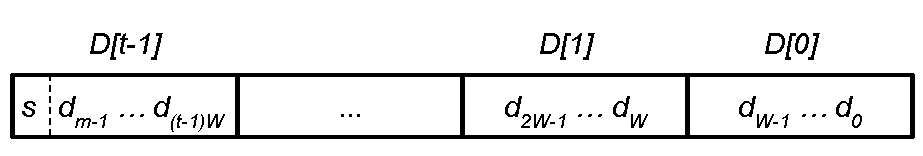
\includegraphics[width = .55\columnwidth]{figures/element-word.pdf}
\end{figure}

This operation has some important practical applications. Using a trinomial as irreducible polynomial is  preferred when available because it maximizes the number of zero coefficients in the the irreducible polynomial, enabling numerous simplifications. And the reduction operation is an important step for multiplications and exponentiations, making speedups desirable.

\section{Operating on words}\label{operating-on-words}

Manipulation of individual bits is not efficient in most CPU architectures. In general, it is preferred to operate on words, with a size specific to the microprocessor architecture, such as $32$- or $64$-bit words. However, the reduction algorithms are strongly bit oriented, since the coefficients are not naturally grouped in words. The codification of these algorithms to word oriented programming languages usually adds some complexity in terms of bitwise shifts and masks, and doesn't enjoy the parallelism inherent in XOR circuits. Specific techniques that help us in this coding have been proposed in the literature\cite{Hilewitz2008}. 

In this scenario it's often desirable to have "interoperability", choosing field sizes and irreducible polynomials that behave well
in both hardware and software implementations. A straightforward
approach to this problem is to develop a hardware implementation first,
XOR'ing individual bits, and convert the algorithm to words. This can be
thought of as parallelizing the operations, with SHIFTs and AND/OR masks
for alignment. This is the approach used in this document.

The word-oriented algorithm can be helped by choosing specific field sizes and irreducible polynomials that introduce operations aligning at word boundaries, to avoid these bitwise shifts and masks, or that map well to architecture-specific operations. In our algorithms we try to make use of alignment opportunities when they appear, but do not depend on them or any specific architecture.